\begin{figure}
    \centering
    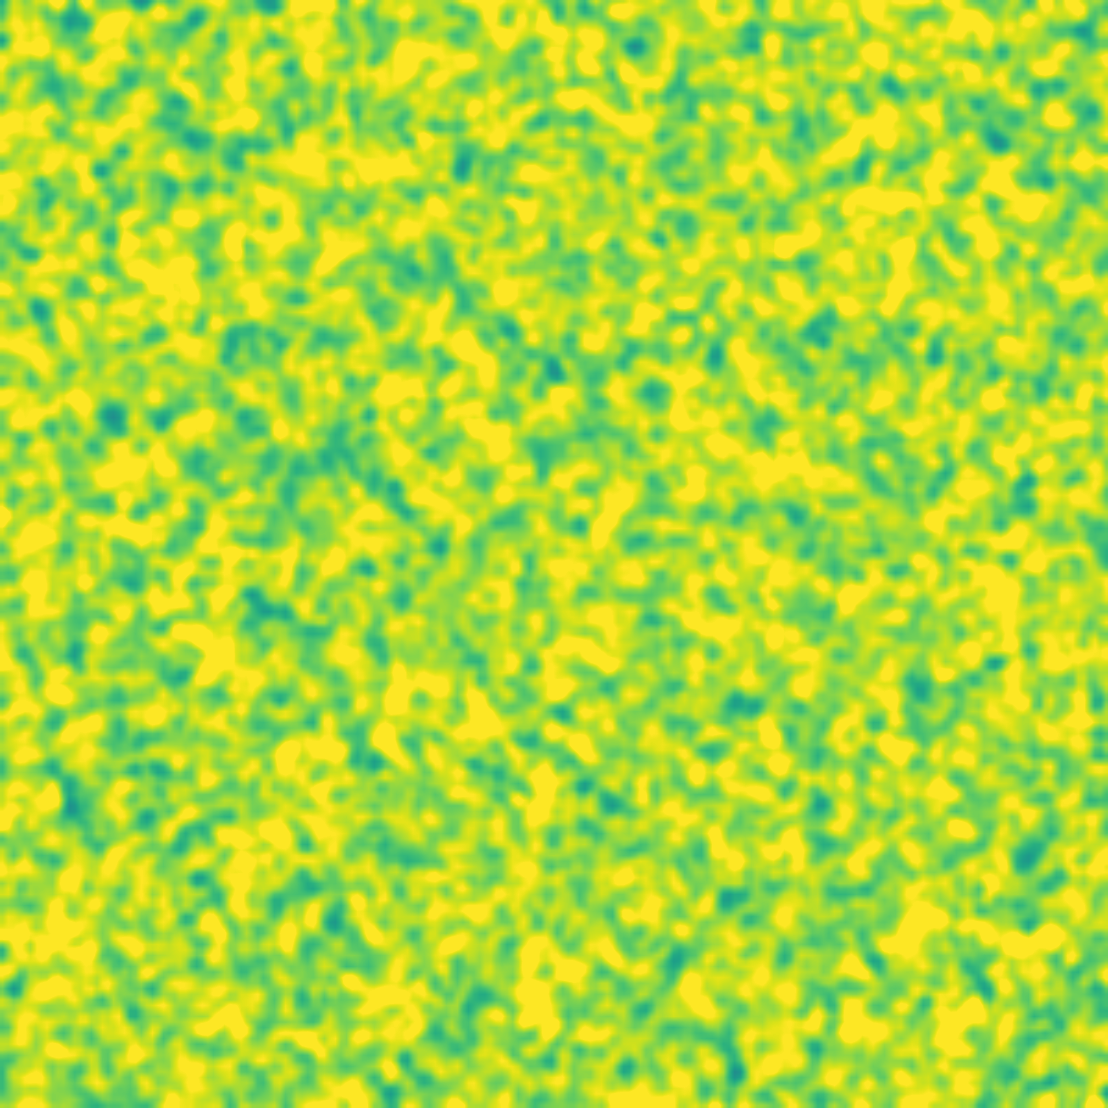
\includegraphics[width=0.32\linewidth]{papers/reaktdiff/images/simpleExample/easy_n1.png}
    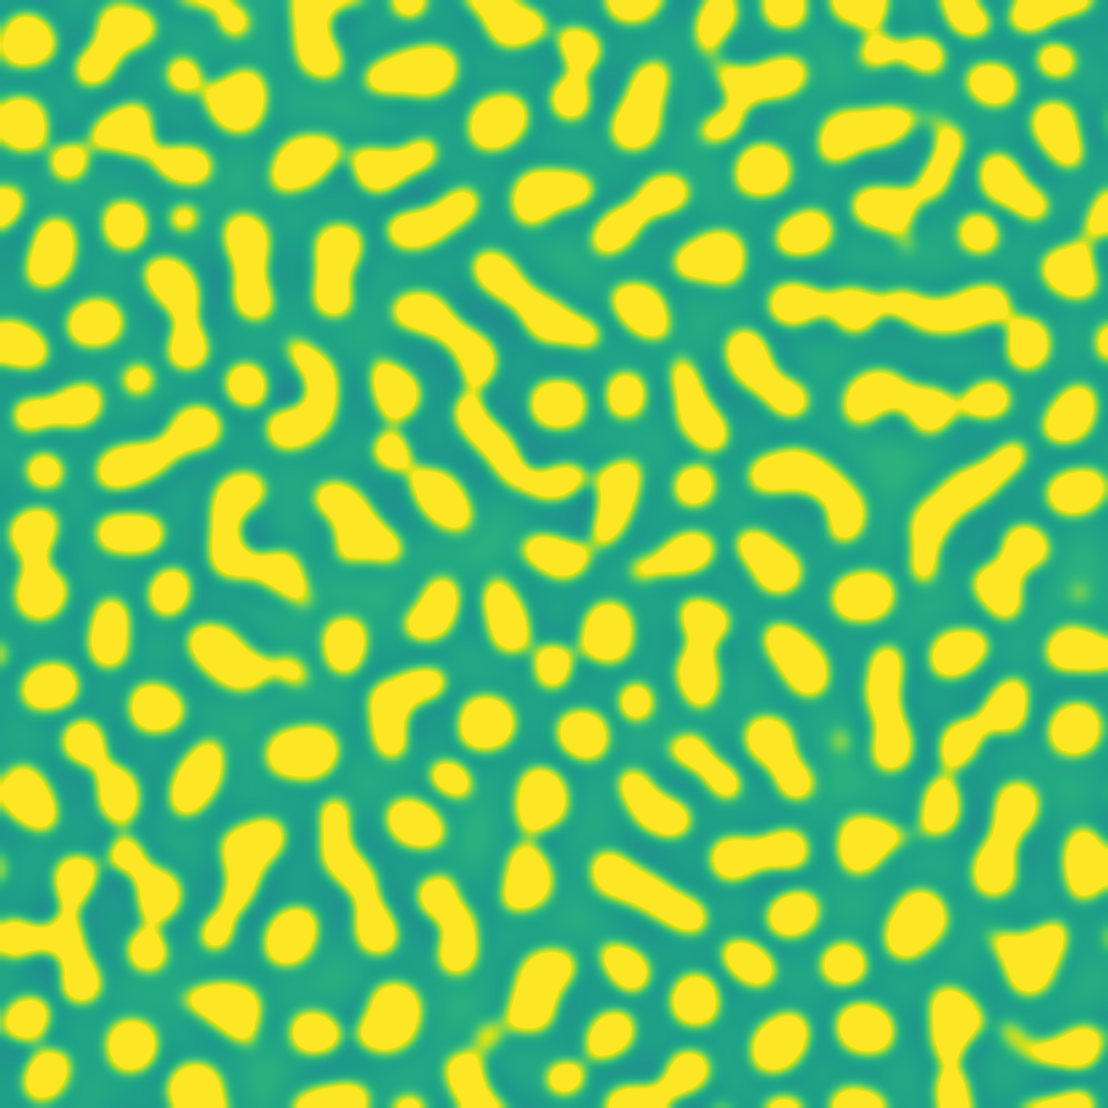
\includegraphics[width=0.32\linewidth]{papers/reaktdiff/images/simpleExample/easy_n300.png}
    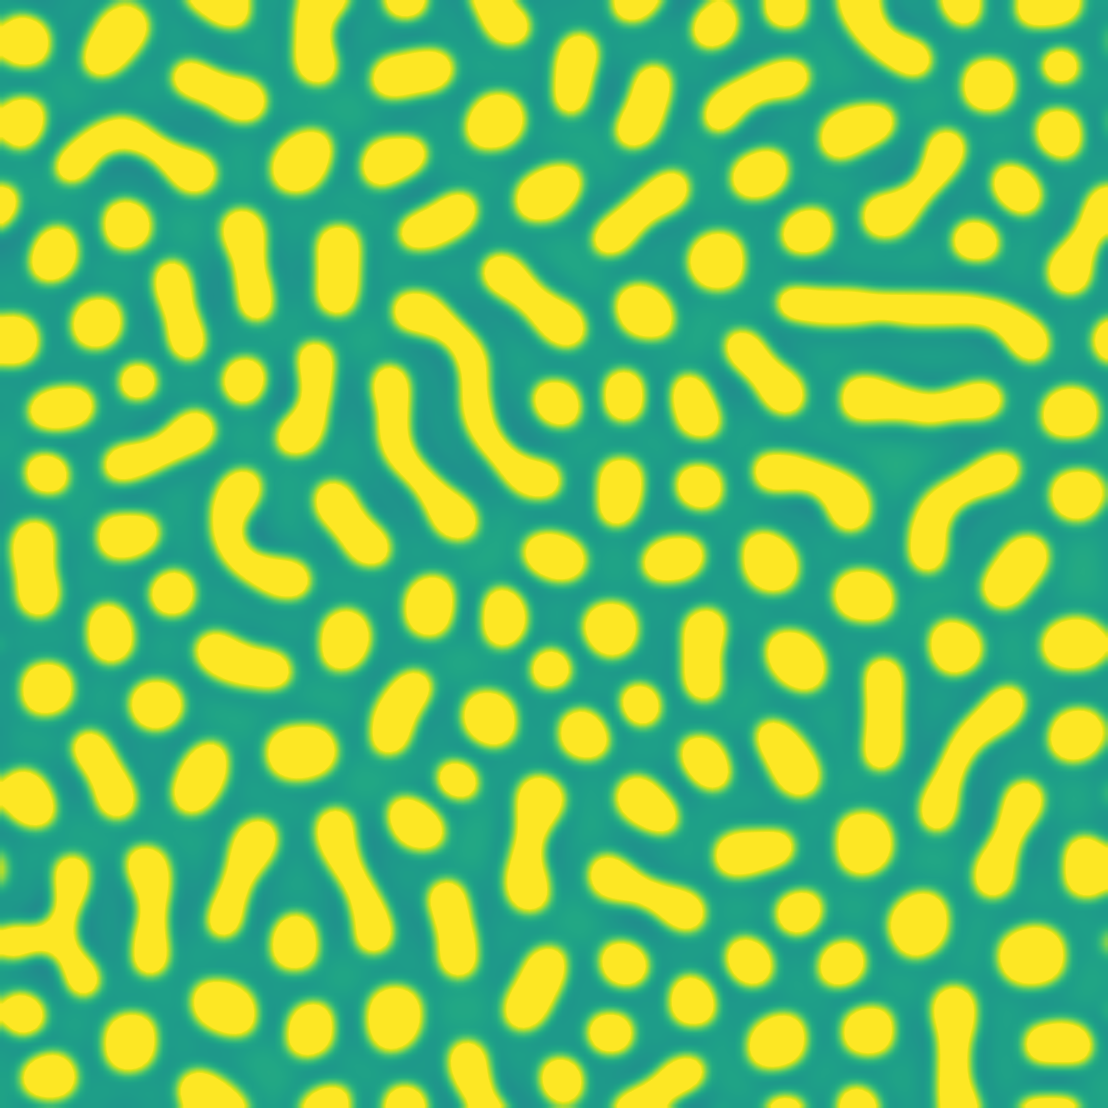
\includegraphics[width=0.32\linewidth]{papers/reaktdiff/images/simpleExample/easy_n999.png}
    \caption{Verlauf der Simulation (von links nach rechts) der Reaktions-Diffusiongleichung mit \eqref{reaktdiff:equ:ownreakterm} als Reaktionsterm}
    \label{reaktdiff:fig:ownreakterm}
\end{figure}
